\chapter{Self-sovereign Identity}\label{chapter: ssi}

% Topic: Identity is extremely important!
Health care, social security, education, access to financial services — this is just a small list of requirements that are essential for a decent life and are usually taken for granted by people in the Western world. Yet, there are more than 1.1 billion people worldwide who cannot provide identification and thus cannot access the most basic services. Digital identities could make a significant contribution towards solving this problem and giving people the chance to participate in society on a more equal playing field. \cite{world_bank_11_2017}

% Topic: We haven't figured it out yet though...
As already mentioned in chapter \ref{chapter: Introduction}, however, current implementations of such digital identities are insufficient for the problems of our modern times. \cite{soltani_survey_2021} divided these problems into four categories:
\begin{enumerate}
	\item Data Ownership and Governance
	\item Password-Based Authentication
	\item Fragmented Identity Data
	\item Data Breaches and Identity Fraud
\end{enumerate}
The former describes the fact that users have no ownership over their digital identities and thus cannot exercise any control over them. Service providers often take advantage of this and use collected data to create comprehensive profiles of their users and thus sell tailored advertising space on corresponding marketplaces for high figures. The lack of control also means that service providers can temporarily or permanently deny users access to their digital identity at any time. At the beginning of 2021, this led to much discussion as the account of former U.S. President Donald Trump was permanently banned from Twitter. One of the central concerns was whether service providers have too much power over users' liberties \cite{noor_should_2021}. In addition, given the frequent and often repeated use of weak passwords, the heavy reliance on password-based authentication is a security risk that may lead to identity theft. If users want to protect themselves, they need to use different and complex passwords for each of their accounts, which quickly becomes a complicated undertaking without a password manager. A study by the password manager LastPass, for example, found that a business customer manages an average of 191 passwords \cite{steel_lastpass_2017}. While the use of such tools greatly simplifies the management of passwords, they too can pose a major security risk and do not completely protect the user \cite{oesch_that_2020, ormandy_password_2021, toth_you_2021}. Alternatives such as \acf{SSO}, where users authenticate to other service providers using for example their Google account, can solve this problem but lead to even greater dependency and centralization. The third issue involves identity data being spread across a large set of service providers, making it difficult to maintain. As a result, duplicates, errors, and outdated data sets are common. The lack of open standards also complicates interoperability between providers, which could theoretically be used to retrieve, move, or delete personal data. Efforts like the Data Transfer Project founded by Microsoft, Google, Twitter, and Facebook try to simplify the transfer of data between providers, but after more than 3 years show very few actual successes \cite{minor_google_2020, hollington_surprising_2021, lomas_facebooks_2020} and are being criticized for pushing small competitors even further behind \cite[p. 15]{borgogno_data_2018}. \cite[pp. 2-3]{soltani_survey_2021}

One of the biggest problems, however, are data breaches. In June 2021 alone, there were 235 breaches with 1.16 billion stolen records, with a total of 18.9 billion records stolen in 1,785 breaches in the first half of 2021 \cite{risk_based_security_data_2021}. Looking at the past, there have been quite a few major hacks \cite{swinhoe_15_2021}, including: 

\begin{itemize}
    \item Yahoo (2013): 3 billion accounts
    \item Marriott (2018): 500 million customer records
    \item Alibaba (2019): 1.1 billion entries
    \item LinkedIn (2021): 700 million accounts
\end{itemize}

A survey of 413 people by \cite{mayer_now_2021} found that 73\% of participants had been affected by at least one, but an average of 5.3 data breaches. In addition, the majority blamed themselves for the breaches, with only 14\% aware that service providers were responsible.

These are decades-old problems that were already critically discussed by Kim Cameron in 2005. Cameron, who last worked as Chief Architect of Identity at Microsoft from 1999 to 2019, wrote the following on a blog article \cite{cameron_laws_2005}:

\begin{displayquote}
    \textit{“The Internet was built without a way to know who and what you are connecting to. This limits what we can do with it and exposes us to growing dangers. If we do nothing, we will face rapidly proliferating episodes of theft and deception that will cumulatively erode public trust in the Internet.”}
\end{displayquote}

Cameron attributes these problems to the lack of an identity layer on the Internet, which has resulted in many services having to find their own solutions. He calls this a \textit{patchwork of identity one-offs}, which fundamentally still exists today and is difficult to resolve. The reason for this, he says, is a lack of consensus and an unwillingness to give up too much control over identity data. A solution for this is, according to him, an \textit{identity metasystem} that abstracts away deeper complexities similar to hardware drivers or TCP/IP and only loosely couples digital identities to the systems.  Such an open identity layer could only be successful if it fulfilled the seven laws of identity defined by Cameron. These include criteria such as user control, consent, pluralism and minimal disclosure. \cite{cameron_laws_2005}

Over the years, these ideas, among others like \cite{marlinspike_what_2012, idcubedorg_id3_2014, allen_path_2016}, gave rise to the concept of \acf{SSI}. It is intended to eliminate the shortcomings of today's established concepts by placing the users in the center and giving them back complete control over their identity data. A user can decide what, to whom and how much data is shared without being dependent on a central authority. The emergence of blockchain technology and various new standards in recent years gave a new boost to implement \ac{SSI} in reality. [\citealp[pp. 6-7]{struker_grundlagen_2021}; \citealp[pp. 8-9]{tobin_inevitable_2017}]

\ac{SSI} is an entirely new approach to digital identities on the Internet and is seen as a paradigm shift that deeply affects the infrastructure and power distribution of the Internet \cite[p. 3]{preukschat_self-sovereign_2021}. For a more profound look at the topic, this chapter takes a closer look at Self-sovereign Identity. To do so, the concept of identity and the different types of identities will be discussed first. This is followed by a historical look at the different stages of digital identities, taking a closer look at the previous concepts of \ac{SSI}. After a basic foundation has been built, standards that have been established in recent years and are intended to make \ac{SSI} feasible in reality are described. Finally, the \ac{SSI} architecture with its components and roles will be looked at.

% Next: Maybe add a short Intro like i did in chapter 1. --> Definition, Motivation, Problem Definition, Vision

    \section{Identity}\label{section: identity}

    What defines a human being? One would probably get various answers to this question, such as its name, gender, place of residence, profession, hobbies, religion, charitable activities, party affiliation or even a combination of all these characteristics. \cite[p. 206]{claus_identity_2001} describes in his work that a person's identity is not just a single, fixed construct, but consists of several partial identities. Thus, depending on the context in which a person finds itself, it takes on one of its various partial identities, which represents it as a human being more or less. For example, a partial identity for health care consists of its medical history, while the partial identity towards work contains received certificates. Nevertheless, these different parts of the identity are not necessarily considered separately, as they can also overlap in certain aspects of information. It is important to mention that a person decides which information to share at which time towards which entity. In figure \ref{figure: alice} the concept of partial identities is illustrated exemplarily by a person Alice.

    An important balancing act is to disclose the right amount of data to maintain anonymity, but also to provide the other person with the necessary information. For the purchase of a water, the kiosk vendor should not ask for any personal data, whereas verification of age when buying alcohol is a valid reason for information disclosure. In reality, official documents, such as state identification documents, or sometimes unofficial documents, such as customer cards, are usually used for such proof of identity. Here, users have full control over their documents as they are under their control, and only they can decide self-sovereignly whom and when to show them. Official identification documents are also produced and standardized to ensure the highest possible level of security and interoperability. Other countries can verify such documents without explicitly contacting authorities, simply by looking at the document. Confidence in the validity of the data arises from the fact that the verifying party trusts the authority issuing the document. \cite[p. 6]{struker_grundlagen_2021}
    
    \begin{figure}[ht]
        \centering
        \makebox[\textwidth]{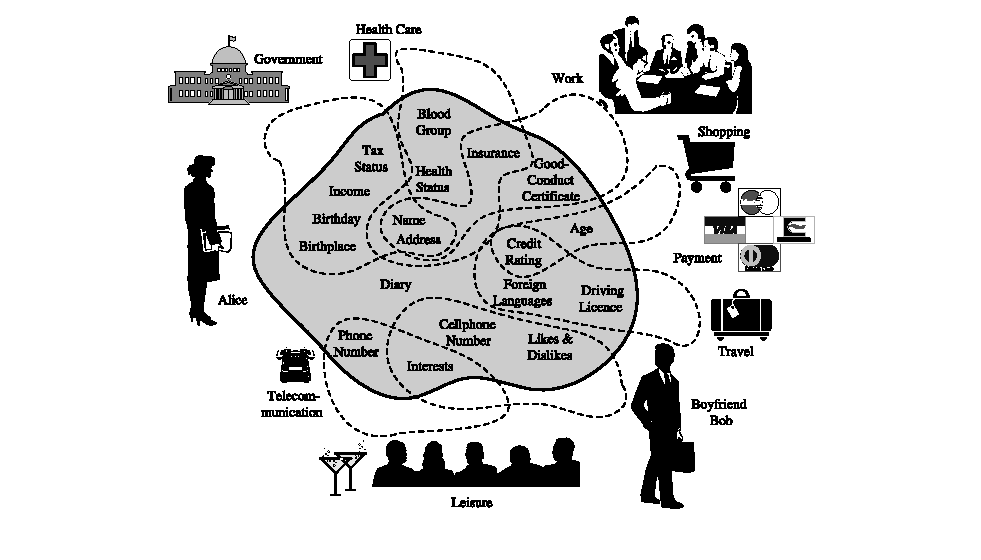
\includegraphics[width=\textwidth]{img/2_alice.eps}}
        \caption{Partial Identities of Alice extracted from \cite{claus_identity_2001}}
        \label{figure: alice}
    \end{figure}

    As a result of the increasing digitalization of various branches of life, many processes are shifting to the digital world. Digital identities, which are similar to analogue identities in terms of their basic idea, are now being used for interacting with digital services. They allow entities, such as people or objects, to authenticate themselves online through certain attributes and thus prove their identity [\citealp[p. 103]{meinel_blockchain_2020}; \citealp{bundesdruckerei_so_2020}]. A more precise definition is given by Cameron \cite{cameron_laws_2005}, who defines digital identity as \textit{“A set of assertions that a digital subject makes about itself or another digital subject”}. In this context, a digital subject is \textit{“A person or thing represented or existing in the digital realm which is being described or dealt with.”} and the attributes mentioned can be represented in the form of claims, which are defined as \textit{“An assertion of the truth of something, typically one which is disputed or doubted”}. The problem is that analogue identities and their documents usually have no or not widely accepted \cite{krempl_e-government-studie_2019, koppenhofer_kabinettsbeschluss_2021} digital representations that could be used as a digital identity. From this emerged the patchwork of identity one-offs described in chapter \ref{chapter: ssi}, resulting in a divergence of digital identities from their original counterparts concerning their characteristics. To better understand this development, the next section describes the different stages of digital identities in more detail. [\citealp[p. 10]{struker_grundlagen_2021}; \citealp[p. 2]{ehrlich_self-sovereign_2021}]
    
	\section{Stages}
	
	As indicated in the last section, Allen's work \cite{allen_path_2016} has had a major influence on what is today considered Self-sovereign Identity and has been cited in over 100 works according to Google Scholar. According to him, digital identities, or online identities, have gone through four major stages since the beginning of the internet. These are examined in more detail below and show which developments led to the emergence of \ac{SSI}.
	
	    \subsection{Centralized Identity}
	    Centralized identities are identities that are issued and verified by a single party or hierarchy. The oldest examples of this are IANA (1988) for the administration of IP addresses, ICANN (1998) for domain names and \acfp{ca}, which play a major role today, particularly in connection with SSL certificates. Especially with the latter, the hierarchical structure of \acp{ca} becomes obvious when one looks at an SSL certificate in the browser. Here, a root authority allows another organization to manage its own hierarchy, while at all times the root authority has full control. This is highly critical for numerous reasons. For example, one entity has complete control over identities and can delete them at any time or even issue false identities. The latter can happen both willingly and unwillingly as a result of a hack. Due to the centralized nature of such authorities, they and thus also the complete hierarchy (chain of trust) are targets of attack, which has been shown in recent years \cite{borchers_diginotar-ssl-gau_2012}. Just like these organizations, due to the lack of an identity layer, all services on the internet developed similar centralized solutions (see chapter \ref{chapter: ssi}. This manifests itself above all in the various accounts that an internet user has to manage for various services. Again, users have little control over their data. \cite{allen_path_2016}
	    
	    \begin{figure}[ht]
    	    \centering
    	    \makebox[\textwidth]{\includesvg[inkscapelatex=false, width=0.6\textwidth]{img/3_central_schema.svg}}
            \caption{Relationship in centralized identities extracted from \cite[p. 7]{preukschat_self-sovereign_2021}}
            \label{figure: centralized}
        \end{figure}
	    
	    In addition, the user has to manage the abundance of login credentials efficiently and securely. However, it is also a challenge for the services, as they have to store a large amount of sensitive data securely and in compliance with data protection laws. Nevertheless, the beneficiaries here are the services, as they can act flexibly and independently of third parties and have full control over the data. \cite[p. 6]{ehrlich_self-sovereign_2021}
	    
	    
	    \subsection{Federated Identity}
	    
	    The second stage of development is represented by the so-called federated identities, which were intended to break down the hierarchies based on a single authority. Here, various commercial organizations developed a model in which control was to be divided between several federated authorities. One of the first projects in this area was Microsoft's Passport in 1999, where Microsoft created a single, federated identity for users that could be used on multiple sites. However, this unification came with the price that Microsoft was now at the center of the federation and could thus exert full control. Other efforts, such as Liberty Alliance Project, founded in 2001, attempted to create an actual federation between multiple companies in which control was distributed among them. The result, however, was a kind of oligarchy in which users still had no control over their data. In the end, the sites remained authorities. \cite{allen_path_2016}
	    
	    \begin{figure}[ht]
    	    \centering
    	    \makebox[\textwidth]{\includesvg[inkscapelatex=false, width=\textwidth]{img/4_federated_schema.svg}}
            \caption{Relationships in federated identities extracted from \cite[p. 8]{preukschat_self-sovereign_2021}}
            \label{figure: federated}
        \end{figure}
	    
	    Nevertheless, this type of digital identity is advantageous in that users do not have to manage an identity/ account for each service and companies have less administrative effort. The identity provider, e.g., Microsoft, acts as the issuer and owner of the data and is thus the central point of contact if a user wants to log on to another service of the federation. The user therefore has no control over his data and is dependent on the continued existence of the identity provider. Due to the abundance of sensitive data, it is possible for the identity provider \ac{IDP} to aggregate information from various areas in order to create user profiles, which in itself can lead to various problems. \cite[pp. 6 - 7]{ehrlich_self-sovereign_2021}
	    
	    \subsection{User-Centric Identity}
	    The goal of user-centric identity is to make federations obsolete and allow the individual to assert control over their identities across multiple authorities \cite{allen_path_2016}. The foundations for this, according to \cite{allen_path_2016}, lie in \cite{jordan_augmented_2003}, in which a \textit{persistent online identity} to be integrated directly into the architecture of the Internet was proposed, making federations unnecessary. One of their central demands was that users should have the right to control their own digital identity. This includes, among other things, the ability to decide what information is collected as part of their digital identity and who has access to which parts. Earlier approaches such as Microsoft's Passport or the Liberty Alliance Project were unable to meet these requirements because, as stated by \cite{jordan_augmented_2003}, they were too business-oriented and thus too focused on the privatization of information. According to them, everyone's digital identities should be a public good that should not be tied to the financial interests of a private company, as their commercial interest may not overlap with those of society. 
	    
	    These thoughts were guiding and influenced various future organizations and initiatives. One influential organization in this area has been the \acf{IIW}, which grew out of efforts by the Identity Commons and the Identity Gang. The \ac{IIW} community played a major role in shaping what is understood by user-centric identity and supported key standards such as OpenID (2005), OpenID 2.0 (2006), OAuth (2010), and OpenID Connect (2014). \cite{allen_path_2016} summarizes the focus of these efforts with the terms user consent and interoperability, which were non-existent or difficult to implement in previous models. These protocols have also been able to achieve significant success when considering the abundance of social logins from for example Facebook, Google, GitHub and Microsoft, which have taken a central position on various websites \cite[p. 8]{preukschat_self-sovereign_2021}. Nevertheless, the original approach of user-centric identities could not be realized further. Like in previous approaches, the identity data and thus absolute control remain with the \ac{SSO} providers who register them. \cite{allen_path_2016} mentions OpenID as an example, which theoretically allows users to set up their own OpenID providers. However, the complexity is so great that in reality this option is hardly ever used. Accordingly, the original problems that user-centric identities were supposed to solve could only be partially solved, since central, mostly private actors have maintained their authority over identity data. Fundamentally, user-centric identities are still federated identities that are now merely interoperable, which is why some literature \cite{ehrlich_self-sovereign_2021, preukschat_self-sovereign_2021} does not list them separately. \cite{allen_path_2016} 
	    
	    \subsection{Self-sovereign Identity}
	    \cite{allen_path_2016} refers to Self-sovereign Identity as the next and most current stage of digital identities, which is intended to solve the issues of all previous stages. In contrast to user-centric identities, users are not only at the center of the identity process, but should also be able to completely own and manage their identities. \cite[p. 12]{preukschat_self-sovereign_2021} describes this as a “[...] shift in control from the centers of the network [...] to the edges of the network [...]”, according to which all users interact directly with each other in a self-sovereign manner as peers. This evolution can be seen in figure \ref{figure: shift}. 
	    
	    \begin{figure}[ht]
    	    \centering
    	    \makebox[\textwidth]{\includesvg[inkscapelatex=false, width=\textwidth]{img/5_shift.svg}}
            \caption{Shift of control with \acs{SSI} extracted from \cite[p. 12]{preukschat_self-sovereign_2021}}
            \label{figure: shift}
        \end{figure}
        
        Apparent here is the new element \textit{registry}, which is used as a (decentralized) public key infrastructure \cite[p. 89]{preukschat_self-sovereign_2021}. A more detailed explanation of this is given in section \ref{section: standards}. To further describe the character of \ac{SSI}, \cite{allen_path_2016} defined 10 principles, with which he connects to previous works like the “Laws of Identity” by \cite{cameron_laws_2005}. These are:
        
        \begin{enumerate}
        	\item Existence: “Users must have an independent existence.”
        	\item Control: “Users must control their identities.”
        	\item Access: “Users must have access to their own data.”
        	\item Transparency: “Systems and algorithms must be transparent.”
        	\item Persistence: “Identities must be long-lived.”
        	\item Portability: “Information and services about identity must be transportable.”
        	\item Interoperability: “Identities should be as widely usable as possible.”
        	\item Consent: “Users must agree to the use of their identity.”
        	\item Minimalization: “Disclosure of claims must be minimized.”
        	\item Protection: “The rights of users must be protected.”
        \end{enumerate}
	    
	    SSI, according to \cite{allen_path_2016}, has its origins in the term “Sovereign Source Authority”, which originated in \cite{marlinspike_what_2012}. In this work, Marlinspike attributes to every human being the right to an identity, which is hindered by tight state structures. In the same year, work began on the Open Mustard Seed by Patric Deegan, which was intended to give users control over their digital identity in a decentralized system. This later resulted in the Windhover Principles (2014), under which the term Self-sovereign Identity appeared \cite{idcubedorg_id3_2014, hub_culture_hubid_2014}. These state, among other things, the following: \cite{allen_path_2016}
	    
	    \begin{displayquote}
            \textit{“Individuals [...] should have control over their digital identities and personal data ensuring trust in our communications, and the integrity of the data we share and transact with. [...] Individuals, not social networks, governments, or corporations, should control their identity credentials and personal data.”}
        \end{displayquote}
        
        Over the course of the following years, \ac{SSI} in connection with blockchain technology was frequently also being discussed in the \ac{IIW} community as well, and various ideas were being developed. This eventually led to some official agencies taking a closer look at this topic. For example, the U.S. Department of Homeland Security Science \& Technology division published a report in 2015 in which it addressed the previously discussed topics by the \ac{IIW}. The EU and countries such as China and Korea have also recognized the potential. In order to make \ac{SSI} implementable in reality, various new standards have been defined over the years in the W3C, among others, which will be discussed in more detail in the next section. \cite[p. 6]{preukschat_self-sovereign_2021}
        
   	\section{Standards}\label{section: standards}
	    In this section, the two most important standards \textit{\acf{DID}} and \textit{\acf{vc}} will be discussed in more detail, as they are the basis for \ac{SSI} and various subsequent standards.
        
	    \subsection{Decentralized Identifier}\label{subsection: did}
	    
	    Throughout history, humans have built up various imaginary networks in which they have to identify and address themselves or objects. Be it physical, mutual networks, in which one identifies itself with one's name or be it postal or telephone networks in which it is the addresses or the telephone numbers. In the age of the Internet, various others have been introduced, such as IP addresses, e-mail addresses, domain names or usernames in social networks. Consequently, there are a large number of identifier systems, which can vary greatly in their nature and place of application. Zooko Wilcox-O'Hearn published an article on this subject in 2001 \cite{wilcox-ohearn_names_2001}, in which he describes a trilemma in identifier systems. According to this, an identifier can probably have at most two of the following properties: \cite[pp. 183-186]{preukschat_self-sovereign_2021}
	    
	    \begin{enumerate}
        	\item Human-readable: Identifiers have semantic meaning in human language and thus have low entropy. 
        	\item Secure: Identifiers are unique and thus bound to a single entity. Spoofing and impersonation should not be possible as well.
        	\item Distributed: The namespace of the identifier is not managed by any central authority. Identifiers can be generated and resolved independently.
        \end{enumerate}
        
        According to this, e-mail addresses, domain names and user names, for example, are human-readable and secure, but do not fulfil the distributed criterion. However, this is precisely what is needed for an SSI ecosystem in which users can own and manage their identity in a self-determined and sovereign manner. With the advent of blockchain technology, however, first solutions emerged that sought to break this problem and thus Zooko's Triangle. This involved the concept of decentralized domain services (see e.g. Namecoin or ENS), with which human-readable, secure and distributed identifiers can be generated. However, these are usually tied to the underlying blockchain and have intrinsic value due to their human-readable nature, which is why domains/ identifiers are often registered and held in such systems without actual use \cite{kalodner_empirical_2015}, questioning the utility of the system.
        
        To meet the requirements related to identifiers in an \ac{SSI} system, the W3C standard \textit{Decentralized Identifier} has been defined. These are \textit{globally unique} and \textit{location-independent} identifiers that can be generated autonomously by entities without central authorities and provide the ability to prove control over them through cryptographic evidence. Regarding Zooko's Triangle, \acp{DID} don't attempt to be human-readable and thus satisfy the properties secure and distributed \cite[p. 185]{preukschat_self-sovereign_2021}. \cite{sporny_decentralized_2021}
        
        The characteristics of a \ac{DID} can be summarized in the following points \cite[p. 160]{preukschat_self-sovereign_2021}: 
        
        \begin{enumerate}
        	\item Persistent: \acp{DID} have no intrinsic expiration date and do not need to change.
        	\item Resolvable: \acp{DID} are resolvable to retrieve additional metadata.
        	\item Cryptographically Verifiable: The owner of a \ac{DID} can cryptographically prove control over it at any time. This is enabled by a public and private key pair being assigned to a \ac{DID}.
        	\item Decentralized: A \ac{DID} \textit{can} be issued/ generated independently of a central authority.
        \end{enumerate}
        
        To better visualize how \acp{DID} work, figure \ref{figure: didArchitecture} provides the \ac{DID} architecture with all its components and relations.
        
        \begin{figure}[ht]
    	    \centering
    	    \makebox[\textwidth]{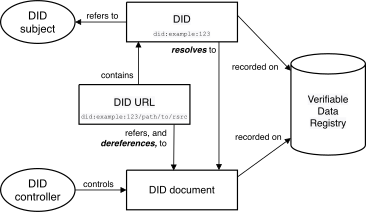
\includegraphics[width=1\textwidth]{thesis/img/8_did_arc.png}}
            \caption{\ac{DID} architecture extracted from \cite{sporny_decentralized_2021} (TODO: VECTOR!)}
            \label{figure: didArchitecture}
        \end{figure}
        
        At the top is the \ac{DID} subject, which can be any entity and is represented by the \ac{DID}. The \ac{DID} itself, for example \texttt{did:example:123456789abcdefghi}, is the actual identifier, which consists of three parts. The first part \texttt{did} describes the identifier schema, \texttt{example} the \ac{DID} method and the third part \texttt{123456789abcdefghi} a \ac{DID} method-specific identifier which can be used to resolve the \ac{DID} document according to the \ac{DID} method. Since \acp{DID} are location-independent, they \textit{can} be recorded in different Verifiable Data Registries, for example blockchains or decentralized file systems. The \ac{DID} method defines any mechanisms for creating, resolving, updating and deactivating \acp{DID} and their \ac{DID} document that may be recorded on a specific data registry. Examples of \ac{DID} methods that rely on blockchains or layers built on top of them as a Verifiable Data Registry include \texttt{did:ethr}, \texttt{did:btcr}, and \texttt{did:ion} which are in contrast to static \ac{DID} methods like \texttt{did:key} which do not require a Verifiable Data Registry and usually wrap the public key from which the DID document can be derived \cite[p. 171]{preukschat_self-sovereign_2021}. The \ac{DID} document contains various metadata about the associated \ac{DID} and define things like verification methods, public keys, and possible service endpoints for interactions with the subject. Additionally, paths can be attached to \acp{DID} to address specific resources within the \ac{DID} document. These are the so-called \ac{DID} URLs. An example \ac{DID} document can be found in listing \ref{listing: didDoc}. \cite{sporny_decentralized_2021}
        \newline
        
        \begin{lstlisting}[language=json, caption={\ac{DID} document example extracted from \cite{sporny_decentralized_2021}}, captionpos=b, label={listing: didDoc}]
{
    "@context": [
      "https://www.w3.org/ns/did/v1",
      "https://w3id.org/security/suites/ed25519-2020/v1"
    ]
    "id": "did:example:123456789abcdefghi",
    "authentication": [{
      "id": "did:example:123456789abcdefghi#keys-1",
      "type": "Ed25519VerificationKey2020",
      "controller": "did:example:123456789abcdefghi",
      "publicKeyMultibase": "zH3C2AVvLMv6gmMNam3uVAjZpfkcJCwDwnZn6z3wXmqPV"
    }]
}\end{lstlisting}
        
        Lastly, figure \ref{figure: didArchitecture} includes the \ac{DID} controller. This is another entity that is authorized to make changes to the \ac{DID} document. Most of the time the \ac{DID} controller is also the \ac{DID} subject, but in some cases these entities can be different (see for example parent-child relationship). \cite{sporny_decentralized_2021}
        
        In conclusion, the \ac{DID} specification is a W3C standard that enables decentralized identifiers for \ac{SSI} ecosystems. The next section presents Verifiable Credentials, which, in conjunction with \acp{DID}, form the basic building blocks of \ac{SSI}.
	    
	    \subsection{Verifiable Credentials}\label{subsection: vc}
	    
	    Now that a standard has been created with \acp{DID}, with which entities can independently generate unique and authority-independent identifiers, there is still a need for a data model with which, in combination with \acp{DID}, identity data can be represented in a standardized way. For this purpose, the W3C defined the \acf{vc} standard. This defines \acp{vc} as a set of claims stated by an issuer in a tamper-evident way, allowing integrity and authorship to be cryptographically verified. A claim is thereby defined, similarly to subsection \ref{section: identity} by Cameron, as an \textit{“[...] assertion made about a subject.”} where a subject is a \textit{“[...] thing about which claims are made.”}. A \ac{vc} is written in JSON-LD and consists of three basic components, which are visualized in figure \ref{figure: vc components}. \cite{sporny_verifiable_2019}
	    
	    \begin{figure}[ht]
    	    \centering
    	    \makebox[\textwidth]{\includesvg[inkscapelatex=false, width=0.5\textwidth]{img/9_vc_components.svg}}
            \caption{Components of \ac{vc} data model extracted from \cite{sporny_verifiable_2019}}
            \label{figure: vc components}
        \end{figure}
        
        The credential metadata can define various properties of the \ac{vc} including its issuer, an expiration date, credential types, or a revocation mechanism that can be used to check whether the issuer has revoked the credential. Thereafter, a set of claims can be defined by the issuer, which contains statements about the subject of the \ac{vc}. Finally, cryptographic proofs can be attached and used to verify the validity of the credential's contents. The standard distinguishes between two types of proofs: \cite{sporny_verifiable_2019}
        
        \begin{enumerate}
            \item External Proof: The contents of the credential are wrapped, thus converted into a different, cryptographically verifiable format. A well-known example of this are JSON web tokens, which are used today in many identity systems for the transfer of claims between multiple parties, providing a certain compatibility to existing systems. Effectively, the set of claims is represented in a digital signature, the JSON web signature. Since these were developed for the JSON format, proofs can only refer to an entire credential and not to individual attribute sets \cite{helmy_jwt_2020}. \cite{sporny_verifiable_2019}

            \item Embedded Proof: The proof is contained in the data and is therefore JOSN-LD native, which makes pre- or post-processing of the data unnecessary \cite{sporny_verifiable_2019}. Such so-called Linked Data Proofs use Linked Data Signatures, which can create proof chains on the basis of the semantic structure of JSON-LD.  This enables proofing on an attribute basis, rather than per credential as in external proofs. This high amount of flexibility also creates room for other technological possibilities, such as zero knowledge proofs. \cite{helmy_jwt_2020}
        \end{enumerate}
        
        In listing \ref{listing: vc example} is an exemplary JSON-LD document, which is leveraging the Verifiable Credentials Data Model, attesting the credential subject a bachelors degree.
        \newline
        
        \begin{lstlisting}[language=json, caption={Example of a Bachelors degree as a Verifiable Credential}, captionpos=b, label={listing: vc example}]  
{
   "@context":[
      "https://www.w3.org/2018/credentials/v1",
      "https://www.w3.org/2018/credentials/examples/v1"
   ],
   "type":[
       "VerifiableCredential",
       "UniversityDegreeCredential"
    ],
    "issuer":{
        "id":"did:key:z6MkhMLpju5tqtbd54BSv7Sq2oRWQo6n..."
    },
    "issuanceDate":"2021-05-26T08:33:40.681Z",
    "credentialSubject":{
       "id":"did:key:z6MkhMLpju5tqtbd54BSv7Sq2oRWQo6n...",
       "type":"BachelorDegree",
       "name":"Bachelor of Science and Arts"
    },
    "proof":{
        "type":"Ed25519Signature2018",
        "created":"2021-05-26T08:33:40Z",
        "jws":"eyJhbGciOiJFZERTQSIsImI2NCI6ZmFsc2UsImNyaXQ...",
        "proofPurpose":"assertionMethod",
        "verificationMethod":"did:key:z6MkhMLpju5tqtbd54BSv7Sq2oRWQo6njMEywrbWAGAp3442#z6MkhM..."
    }
}\end{lstlisting}
	   
	   Listing \ref{listing: vc example} also shows the basic building blocks described earlier. The document starts with a context definition to reference the semantic vocabulary. This is followed by a definition of the credential types, the issuer and the issuing time (credentials metadata). After that follows the actual claim in the object \texttt{credentialSubject}, where the subject and the corresponding degree are defined. At this point it also becomes clear how the \ac{DID} and \ac{vc} specifications are intertwined: both issuer and subject are defined by their DID.  The public private key pair belonging the issuer's DID becomes relevant especially in the next point: the proof. Here, the issuer uses the private key coupled to its DID to generate the Linked Data signature and thus makes the credential verifiable.
	   
	   Another important part of the standard are \acfp{VP}. If a holder of a Verifiable Credential wants to present it to someone, it can combine one or more \acp{vc} in a Verifiable Presentation without invalidating the cryptographic proofs. This approach has several advantages. On the one hand, the owner of the credential can specify granularly which credentials it wants to disclose and, at the same time, a type of proof of ownership can be provided. This becomes particularly clear if one considers the structure of such a \ac{VP} in figure \ref{figure: vp components}. \cite{sporny_verifiable_2019}
	   
	   \begin{figure}[ht]
    	    \centering
    	    \makebox[\textwidth]{\includesvg[inkscapelatex=false, width=0.5\textwidth]{img/10_vp_components.svg}}
            \caption{Components of a Verifiable Presentation extracted from \cite{sporny_verifiable_2019}}
            \label{figure: vp components}
        \end{figure}
        
        Once again, metadata is defined at the beginning, which can include attributes like the context and types. This is followed by the \acp{vc} to be presented, which are listed directly one after the other without any changes. Finally, a cryptographic proof follows, which the owner of the credentials generates with the private key of its \ac{DID}. This protects the integrity of the presentation and at the same time certifies that the credentials are actually presented by the owner of the \ac{DID}. The inclusion of the attributes \texttt{challenge} and \texttt{domain} in the proof can also provide protection against replay attacks, in which an attacker presents the intercepted presentation again to another verifier without authorization. \cite{sporny_verifiable_2019}
        
        Having introduced Decentralized Identifiers and Verifiable Credentials as the backbone of an \ac{SSI} ecosystem, the next section will specify a few things in more detail.
	   
    \section{Architecture}
        In this section, various functional aspects of \ac{SSI} are described in more detail. For this purpose, the roles and interactions in a \ac{SSI} system are described, followed by a general look at the technology stack.
        
    	\subsection{Roles}
    	
    	In an SSI ecosystem, there are three basic roles that participants can occupy: issuer, verifier, and holder. They have already been briefly described in subsection \ref{subsection: vc} and are therefore an integral part of the \ac{vc} standard. The three roles are briefly presented below: [\citealp[pp. 25-26]{preukschat_self-sovereign_2021}; \citealp{sporny_verifiable_2019}]
    	
    	\begin{enumerate}
        	\item \textit{Issuer}: An entity that makes statements within a \ac{vc} about a subject. Such an entity can be organizations such as governments, universities, but also private individuals or objects such as sensors. An issuer transmits \acp{vc} to holders.
        	\item \textit{Holder}: An entity that requests or receives \acp{vc} from issuers and manages them in a credential repository/ digital wallet. However, a holder may not always be the (credential) subject. Examples of these cases include a parent (holder) holding \acp{vc} for its child (subject) or a friend (holder) filling a prescription at the pharmacy for its sick friend (subject). Holders can also generate Presentations from Verifiable Credentials and show them to a verifier.  
        	\item \textit{Verifier}: An entity that wants to verify certain attributes or claims of a subject. It may receive these in the form of \ac{VP}, which may contain those claims from one or more \acp{vc}. However, holders have control at all times over which attributes are passed to the verifier.
        \end{enumerate}
        
        The roles and their relations are often called the trust triangle, as it describes how trust is formed in an \ac{SSI} ecosystem. Like in the real world, trust in the credentials comes from a verifier trusting the issuer. The figure \ref{figure: vc lifecycle} shows this triangle, but also visualizes how the roles interact with \acp{vc}, which is why this process is also called the Verifiable Credential Lifecycle. [\citealp[pp. 25-26]{preukschat_self-sovereign_2021}; \citealp{sporny_verifiable_2019}]
        
        \begin{figure}[htp]
    	    \centering
    	    \makebox[\textwidth]{\includesvg[inkscapelatex=false, width=0.75\textwidth]{img/11_vc_lifecycle.svg}}
            \caption{Verifiable Credential Lifecycle edited and extracted from \cite{sporny_verifiable_2019}}
            \label{figure: vc lifecycle}
        \end{figure}
        
        The lifecycle shows which phases a Verifiable Credential goes through and which roles perform which actions in these phases. At this point, the process is described using a Verifiable Credential representing a bachelor's degree as an example. Here, the issuer is a university, the holder is an alumnus, and the verifier is a potential employer. The process is as follows:  \cite{sporny_verifiable_2019}
        
        \begin{enumerate}
            \item \textit{Issue}: The now alumnus has successfully defended its thesis. Its university then issues a Verifiable Credential to the \ac{DID} of the alumnus with its own \ac{DID}. As holder and subject, the alumnus stores the \ac{vc} in its digital wallet.
            \item \textit{Transfer}: The alumnus can transfer this \ac{vc} to another holder, e.g., if he authorizes a friend to go to a governmental authority for him with the degree.
            \item \textit{Present}: The alumnus presents the \ac{vc} of the bachelor's degree, optionally inside a \ac{VP}, to the potential employer as part of his application in order to have his degree verified.
            \item \textit{Verify \& Check Status}: The potential employer checks the authenticity of the credential. This includes firstly checking that the credential meets the standard, the proofs are valid and is not revoked. To check the proof, the employer must resolve the \ac{DID} documents of the \acp{DID} in the credential to obtain the public keys. For this, depending on the DID methods used, the employer may need to query a verifiable data registry (see subsection \ref{subsection: did}. 
            \item \textit{Revoke}: If the university wants to revoke and thus invalidate a \ac{vc} for some reason, it can do so. Depending on the implementation, this is also done with some kind of decentralized or central registry. One of them is described later on in subsection \ref{subsection: revocationlist2020}.
            \item \textit{Delete}: A holder can delete a \ac{vc} from its digital wallet at any time, which does not affect its overall validity.
        \end{enumerate}
        
        This process can be applied to any other use case and creates a system through defined standards, technologies and the described trust model, which in its basic characteristics also takes place in real interactions and where trust can form between entities.
        
    	\subsection{Technology Stack}
    	
    	Looking at the \ac{SSI} technology stack, figure \ref{figure: ssi_stack_detail} provides an overview that divides it into five basic layers. This is based on previous work from the Decentralized Identity Foundation and the Trust over IP organization \cite{heck_ssi_2020,hakan_yildiz_layers_2021, davie_0289_2021}. A notable change is that here the communication layer has been broken out of the agent layer. Even though it is mostly used by agents, it's not part of the agents itself, but rather an implemented software module leveraging the communication layer.
    	
		\begin{figure}[h]
            \centering
            \makebox[\textwidth]{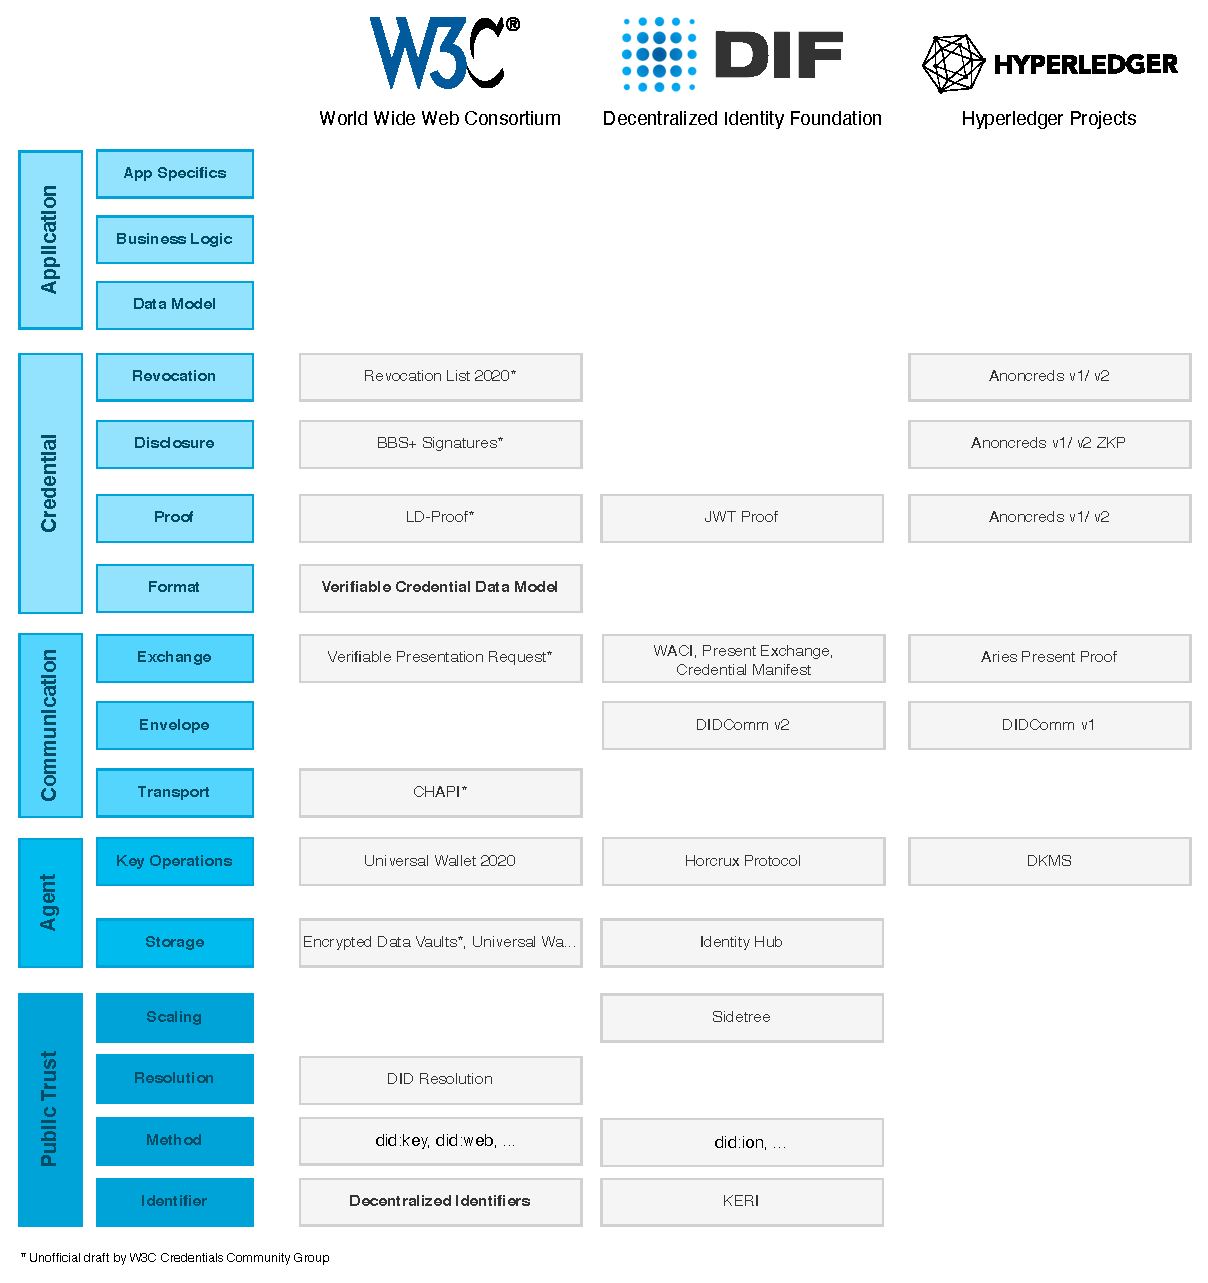
\includegraphics[width=0.9\textwidth]{img/7_arch_detail.eps}}
            \caption{\ac{SSI} technology stack, standards, and efforts based on  \cite{heck_ssi_2020,hakan_yildiz_layers_2021,davie_0289_2021}}
            \label{figure: ssi_stack_detail}
        \end{figure}
        
        The public trust layer is the baseline layer and thus forms the basis for all other layers above it. The aim here is to create a public trust registry that includes, for example, DIDs and their DID methods and thus serves as a (decentralized) public key infrastructure. As already mentioned, this may or may not imply the need for technologies like blockchains or decentralized file systems. In the subsequent agent layer, which fundamentally allows an entity to \textit{“[...] take actions, perform communications, store information, and track usage of the digital wallet.”} \cite[p. 192]{preukschat_self-sovereign_2021} and thus handles tasks related to storing \acp{vc} and \acp{DID} and performing key operations. This includes for example the generation of proofs, but also the deactivation or generation of new key pairs. On top of this is the communication layer, which handles the communication between agents. This includes transport, envelope, and credential exchange standards and protocols. On the fourth level is the credential layer, which includes all standards and technology used in the credentials' data model, such as formats, types of proofs, disclosure, and revocation. The top level is the application layer, which creates user applications based on the underlying layers that cover and implement specific use cases. This includes concrete data models for the credentials, but also business and application-specific logic and technology. \cite{heck_ssi_2020,hakan_yildiz_layers_2021, davie_0289_2021, preukschat_self-sovereign_2021}
        
        In addition to the general structure and elements of the layers, figure \ref{figure: ssi_stack_detail} contains concrete standards and community efforts which provide the layers with a technological basis. A differentiation is made here between the concrete efforts of the three most important organizations in this area. It should be noted at this point that this overview does not claim to be complete and is merely illustrative.
		
	\section{Recent Developments}
		\subsection{DIDComm}
		\subsection{Zero Knowledge Proofs}
		\subsection{RevocationList2020}\label{subsection: revocationlist2020}